\documentclass[12pt]{article}
\usepackage{graphicx}
\usepackage{gensymb}
\usepackage[none]{hyphenat}
\usepackage{graphicx}
\usepackage{listings}
\usepackage[english]{babel}
\usepackage{graphicx}
\usepackage{caption}
\usepackage{hyperref}
\usepackage{booktabs}
\usepackage{array}
\usepackage{amsmath}
\usepackage{listings}
\graphicspath {./sdcard/fwc/}
\lstset{
        frame=single'
	breaklines=true
	}
\newcommand{\mydet}[1]{\ensuremath{\begin{vmatrix}#1\end{vmatrix}}}
\providecommand{\brak}[1]{\ensuremath{\left(#1\right)}}
\providecommand{\norm}[1]{\left\lVert#1\right\rVert}
\newcommand{\solution}{\noindent \textbf{Solution: }}
\newcommand{\myvec}[1]{\ensuremath{\begin{pmatrix}#1\end{pmatrix}}}
\let\vec\mathbf	

\begin{document}
\begin{center}
\textbf\large{CHAPTER - 9  \\  TRIANGLES}
\section*{EXERCISE - 9.4}
\end{center}

\begin{enumerate}

\item A point $\vec{E} $ is taken on the side $BC$ of a parallelogram ABCD.$AE$ and  $DC$ are produced to meet at $\vec{F}$.Prove that  $ar (ADF) = ar (ABFC)$.
\item The diagonals of a parallelogram ABCD intersect at a point $\vec{O}$.Through $\vec{O}$,a line is drawn to intersect $AD$ at $\vec{P}$ and $BC$ at $\vec{Q}$.Show that $PQ$ divides the parallelogram into two parts of equal area.
\item The medians $BE$ and $CF$ of a triangle ABC intersect at $\vec{G}$.Prove that the area of $ \triangle${GBC}= area of the quadrilateral AFGE.	
\item In Fig.\ref{fig:9.24},$CD \parallel AE$  and $CY \parallel BA$.Prove that  $ar (CBX) =  ar (AXY)$
\begin{figure}[h]
	\centering
	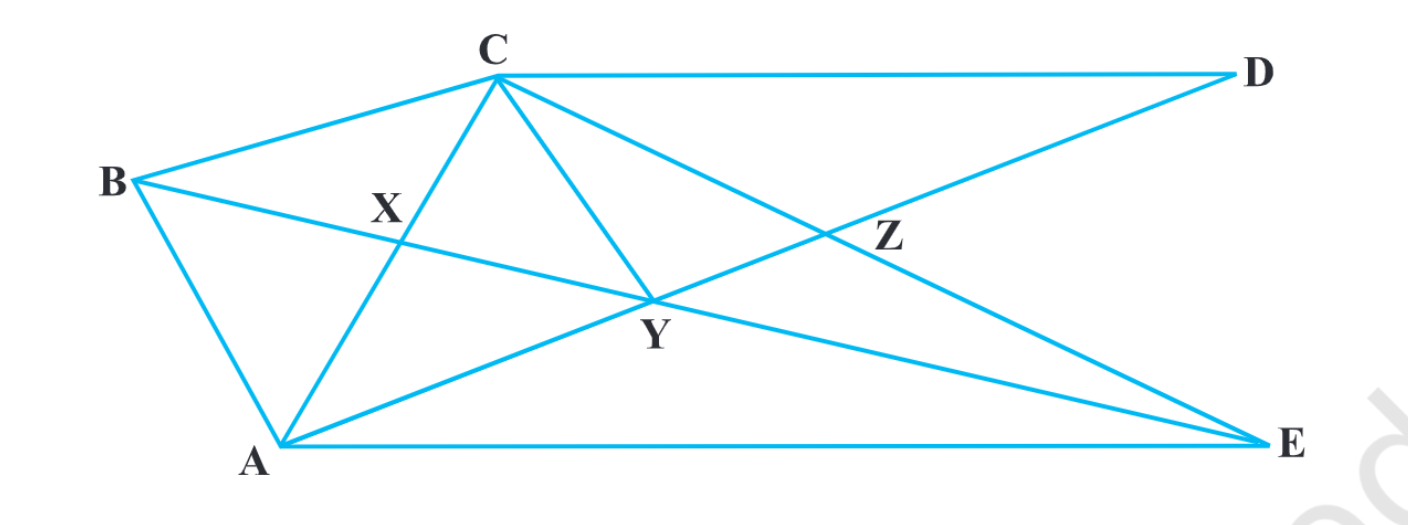
\includegraphics[width=\columnwidth]{figs/Fig9.24.png}
	\caption{}
	\label{fig:9.24}
\end{figure}
\item ABCD is a trapezium in which $AB \parallel DC$,$DC = 30cm$  and $AB = 50cm$.If $\vec{X}$ and $\vec{Y}$ are,respectively the mid-points of $AD$ and $BC$,prove that  $ar (DCYX) = \frac{7}{9} ar (XYBA)$.
\item  In $ \triangle${ABC},if $\vec{L}$ and $\vec{M}$ are the points on $AB$ and $AC$,respectively such that $LM \parallel BC$.Prove that $ar (LOB) = ar (MOC)$.
\item In Fig.\ref{fig:9.25},ABCDE is any pentagon.$BP$ drawn parallel to $AC$ meets $DC$ produced at $\vec{P}$ and $EQ$ drawn parallel to $AD$ meets $CD$ produced at $\vec{Q}$.Prove that  $ ar (ABCDE) = ar (APQ) $.
\begin{figure}[h]
	\centering
	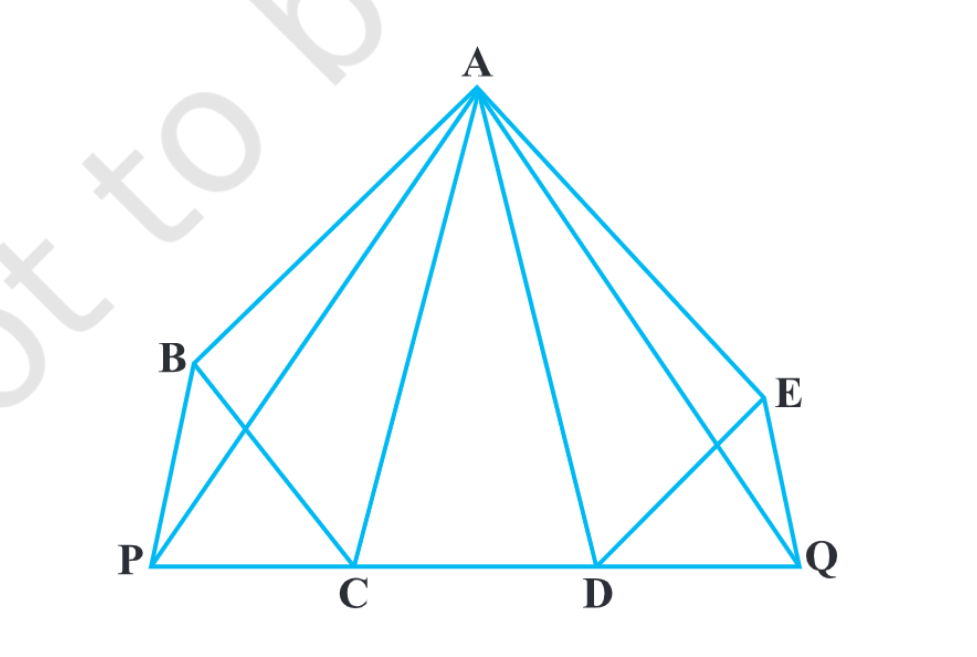
\includegraphics[width=\columnwidth]{figs/Fig9.25.png}
	\caption{}
	\label{fig:9.25}
\end{figure}
\item If the medians of a $ \triangle$ ABC  intersect at $\vec{G}$,show that
	\begin{align} 
		{ar (AGB)} &={ar (AGC)}= {ar (BGC)} = \frac{1}{3} {ar (ABC)}
	\end{align}
\item In Fig.\ref{fig:9.26},$\vec{X}$ and $\vec{Y}$ are the mid-points of $AC$ and $AB$ respectively,$QP \parallel BC$ and $CYQ$ and $BXP$ are straight lines.Prove that $ ar (ABP) = ar (ACQ) $.
\begin{figure}[h]
	\centering
	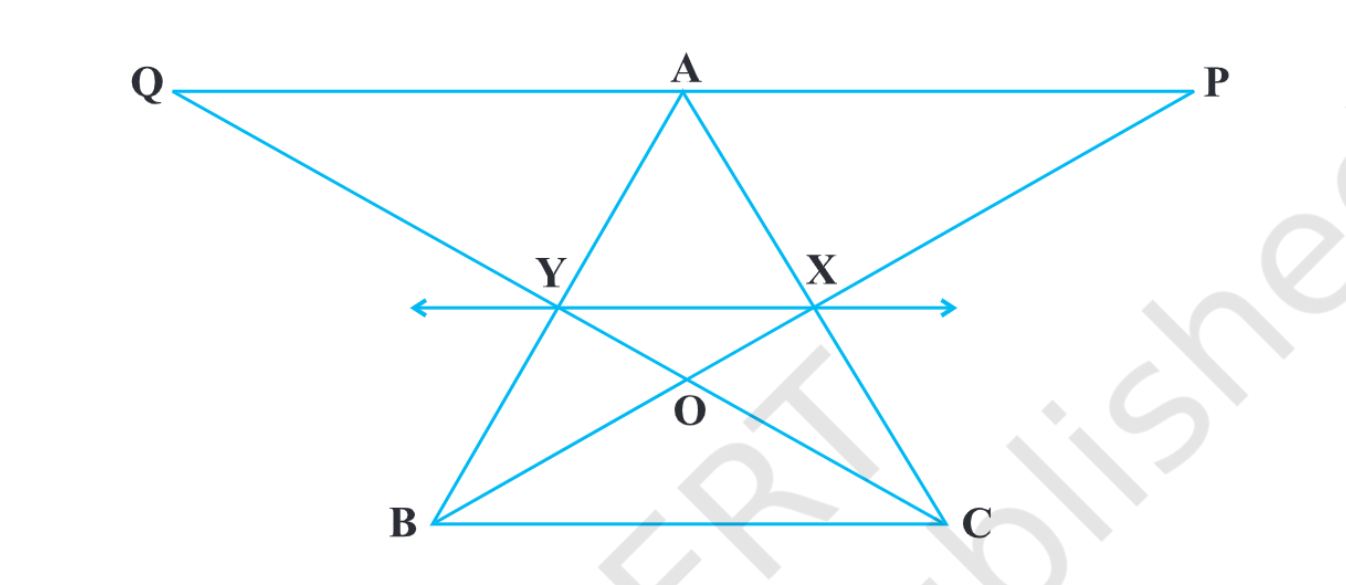
\includegraphics[width=\columnwidth]{figs/Fig9.26.png}
	\caption{}
	\label{fig:9.26}
\end{figure}
\item In Fig.\ref{fig:9.27},ABCD and AEFD are two parallelograms.Prove that $ ar (PEA) = ar (QFD) $ [Hint:Join PD].
\begin{figure}[h]
	\centering
	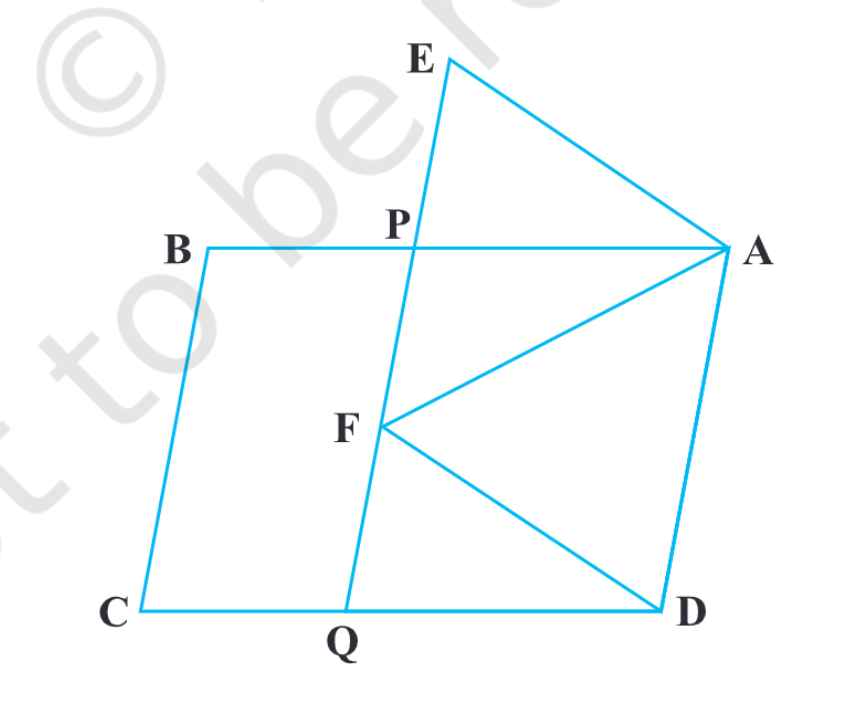
\includegraphics[width=\columnwidth]{figs/Fig9.27.png}
	\caption{}
	\label{fig:9.27}
\end{figure}
\end{enumerate}
\end{document} 
